\documentclass[11pt]{article}
\usepackage[margin=1in]{geometry}
\usepackage{booktabs}
\usepackage{graphicx}
\usepackage{amsmath}

\title{CloSeNet Ablation Report}
\date{}

\begin{document}
\maketitle
\sloppy

\section{Headline Results}

Mean $\pm$ std across 3 seeds for all 10 ablations, on mIoU, freq\_IoU, B-IoU,
mIoU@boundary, mIoU@inner, and segm\_loss. The best value per column is bolded. This
table is the anchor of the paper -- everything else supports it. Since B-IoU is the
headline metric, a $\Delta$ B-IoU vs.\ baseline column is also reported.

\begin{table}[h]
\centering
\resizebox{\textwidth}{!}{\begin{tabular}{lccccccc}
\toprule
Model & mIoU & freq\_IoU & B-IoU & mIoU@boundary & mIoU@inner & segm\_loss & $\Delta$ B-IoU vs.\ baseline \\
\midrule
CloSeNet & 89.26 $\pm$ 0.13 & 91.59 $\pm$ 0.42 & \textbf{81.43 $\pm$ 0.85} & 88.26 $\pm$ 0.14 & \textbf{99.22 $\pm$ 0.09} & \textbf{0.1347 $\pm$ 0.0052} & -- \\
+ CBL & 89.28 $\pm$ 0.22 & 91.26 $\pm$ 0.22 & 80.90 $\pm$ 1.19 & 88.26 $\pm$ 0.28 & 99.06 $\pm$ 0.19 & 0.1370 $\pm$ 0.0066 & -0.53 \\
+ PTB & 90.91 $\pm$ 0.19 & 92.10 $\pm$ 0.17 & 77.85 $\pm$ 0.37 & 89.98 $\pm$ 0.21 & 98.91 $\pm$ 0.13 & 0.1443 $\pm$ 0.0011 & -3.59 \\
+ PTB + SegFix & 91.08 $\pm$ 0.15 & 91.89 $\pm$ 0.12 & 77.85 $\pm$ 0.29 & 90.19 $\pm$ 0.20 & 98.81 $\pm$ 0.16 & 0.1469 $\pm$ 0.0026 & -3.58 \\
+ PTB + CBL & 91.08 $\pm$ 0.22 & 91.86 $\pm$ 0.27 & 77.54 $\pm$ 0.12 & 90.14 $\pm$ 0.20 & 98.73 $\pm$ 0.17 & 0.1488 $\pm$ 0.0045 & -3.89 \\
+ PTB + CBL + SegFix & 91.04 $\pm$ 0.06 & 91.78 $\pm$ 0.16 & 77.51 $\pm$ 0.35 & 90.20 $\pm$ 0.11 & 98.84 $\pm$ 0.21 & 0.1506 $\pm$ 0.0048 & -3.92 \\
+ PTB + BRM & 91.16 $\pm$ 0.42 & 92.10 $\pm$ 0.44 & 77.27 $\pm$ 0.27 & 90.17 $\pm$ 0.42 & 99.05 $\pm$ 0.14 & 0.1682 $\pm$ 0.0116 & -4.16 \\
+ PTB + BRM + SegFix & 90.80 $\pm$ 0.08 & 91.74 $\pm$ 0.14 & 76.90 $\pm$ 0.33 & 89.91 $\pm$ 0.07 & 99.04 $\pm$ 0.05 & 0.1674 $\pm$ 0.0102 & -4.54 \\
+ PTB + BRM + CBL & \textbf{91.21 $\pm$ 0.28} & \textbf{92.11 $\pm$ 0.10} & 77.24 $\pm$ 0.31 & \textbf{90.23 $\pm$ 0.31} & 98.96 $\pm$ 0.13 & 0.1650 $\pm$ 0.0053 & -4.19 \\
+ PTB + BRM + CBL + SegFix & 91.01 $\pm$ 0.07 & 91.76 $\pm$ 0.36 & 77.14 $\pm$ 0.48 & 90.18 $\pm$ 0.11 & 99.00 $\pm$ 0.10 & 0.1639 $\pm$ 0.0034 & -4.30 \\
\bottomrule
\end{tabular}
}
\end{table}

\section{CBL $\times$ PTB Factorial}

This is the central scientific claim: does combining CBL and PTB help more, less, or
the same as their individual effects would predict? The interaction plot below shows
the four cells (baseline, +CBL, +PTB, +CBL+PTB) as two lines -- \{no CBL, +CBL\} --
over \{no PTB, +PTB\}, for both B-IoU and mIoU, with error bars from seed std.
Parallel lines indicate additive (independent) effects; crossing or diverging lines
indicate an interaction.

\begin{figure}[h]
\centering
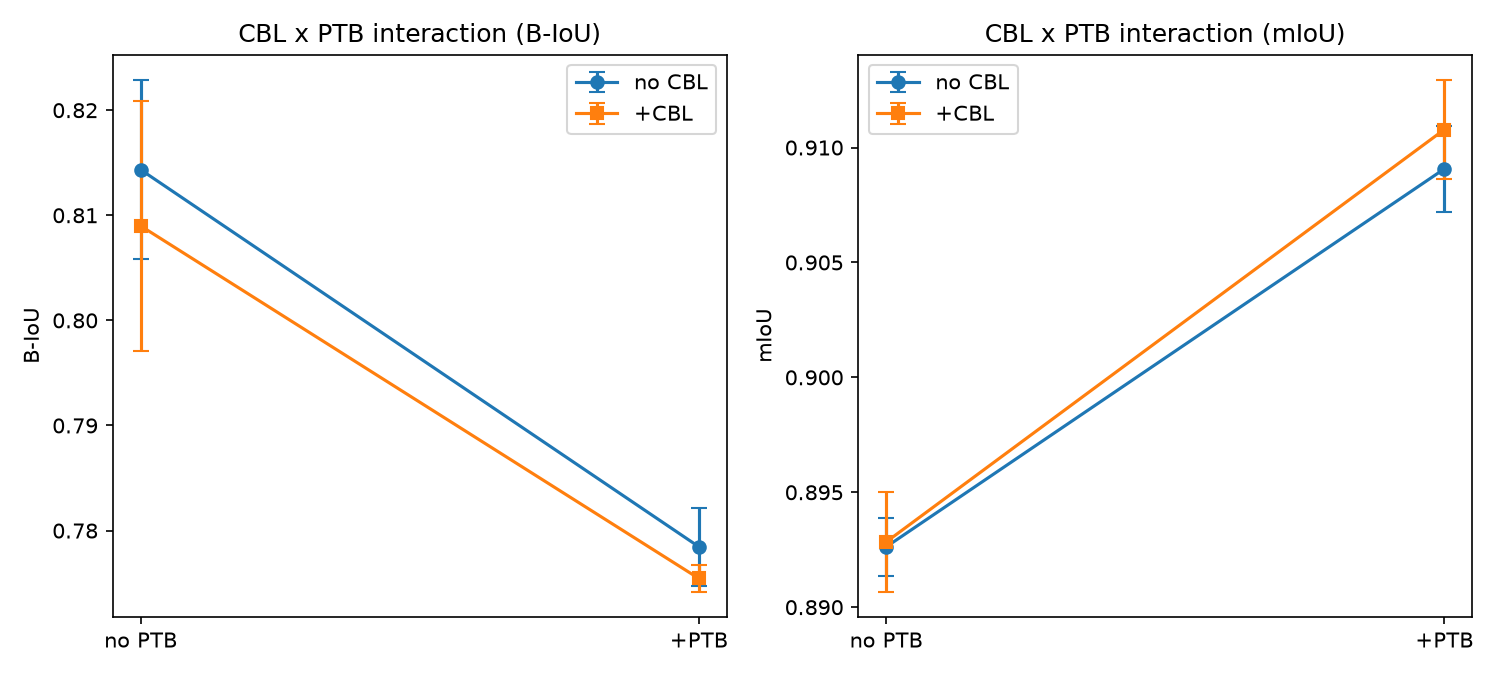
\includegraphics[width=\linewidth]{figures/interaction_cbl_ptb.png}
\caption{CBL $\times$ PTB interaction plot (error bars: seed std).}
\end{figure}

The table below is the quantitative version of the plot: the main effect of CBL
(average of CBL rows minus non-CBL rows), the main effect of PTB (average of PTB
rows minus non-PTB rows), and the interaction term
$(\text{PTB+CBL} - \text{PTB}) - (\text{CBL} - \text{baseline})$, each reported as
mean $\pm$ std across the 3 matched seeds. Where an effect is smaller than 2$\times$
its std, the cell states ``no detectable effect at $n{=}3$ seeds'' rather than
reporting a possibly spurious sign.

\begin{table}[h]
\centering
\begin{tabular}{lcc}
\toprule
Effect & B-IoU & mIoU \\
\midrule
CBL main effect & no detectable effect at $n{=}3$ seeds & no detectable effect at $n{=}3$ seeds \\
PTB main effect & no detectable effect at $n{=}3$ seeds & no detectable effect at $n{=}3$ seeds \\
Interaction & no detectable effect at $n{=}3$ seeds & no detectable effect at $n{=}3$ seeds \\
\bottomrule
\end{tabular}

\end{table}

\section{BRM Results}

This is the likely headline finding: does the Boundary-aware Refinement Module,
combined with CBL, beat PTB alone, PTB+CBL, and PTB+BRM individually? PTB+BRM+CBL does not clearly beat every comparison on B-IoU (see: PTB+BRM+CBL vs.\ PTB, PTB+BRM+CBL vs.\ PTB+CBL, PTB+BRM+CBL vs.\ PTB+BRM).
The synergy claim being tested is whether adding CBL on top of BRM specifically
helps more than adding CBL elsewhere (compare the CBL main effect from Section 2 to
the PTB+BRM+CBL vs.\ PTB+BRM row below).

\begin{figure}[h]
\centering
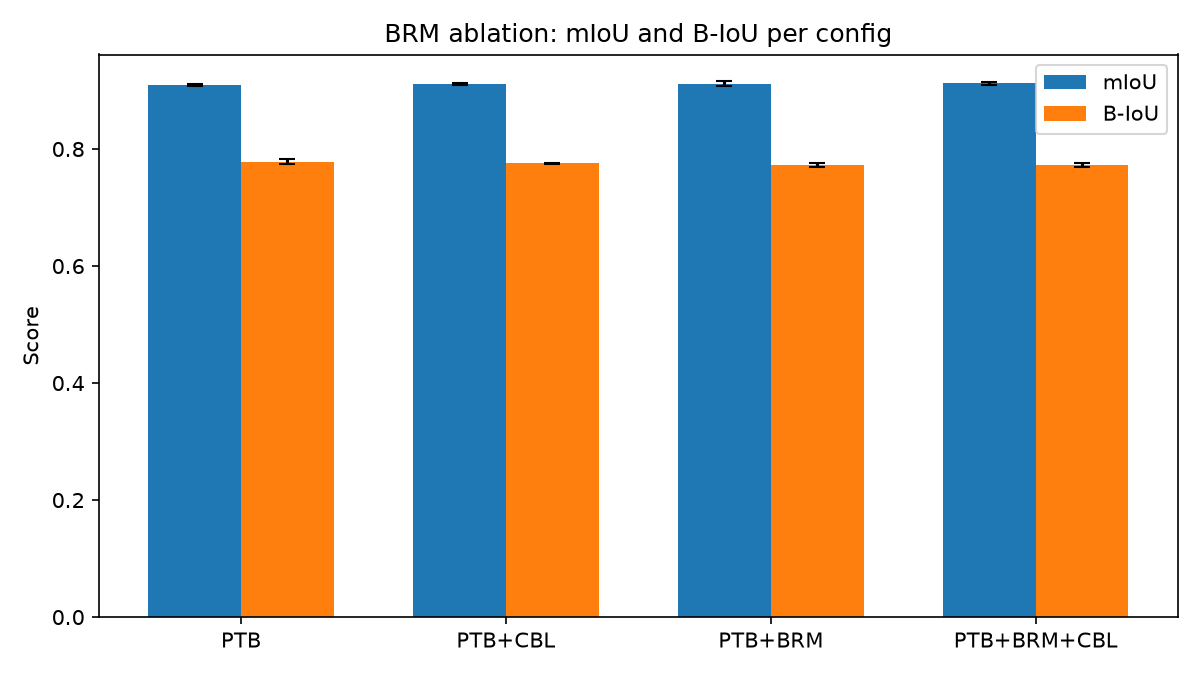
\includegraphics[width=0.8\linewidth]{figures/brm_grouped_bars.png}
\caption{mIoU and B-IoU per PTB-family config, error bars: seed std.}
\end{figure}

\begin{table}[h]
\centering
\resizebox{\textwidth}{!}{\begin{tabular}{lcc}
\toprule
Comparison & B-IoU & mIoU \\
\midrule
PTB+BRM+CBL vs.\ PTB & no detectable effect at $n{=}3$ seeds & +0.30 $\pm$ 0.11 \\
PTB+BRM+CBL vs.\ PTB+CBL & no detectable effect at $n{=}3$ seeds & no detectable effect at $n{=}3$ seeds \\
PTB+BRM+CBL vs.\ PTB+BRM & no detectable effect at $n{=}3$ seeds & no detectable effect at $n{=}3$ seeds \\
\bottomrule
\end{tabular}
}
\end{table}

\section{SegFix Post-Processing Effect}

Does post-processing help uniformly, or does its benefit shrink once the model
itself is already boundary-aware? Going from PTB to PTB+BRM+CBL, the SegFix B-IoU delta is not monotonic (PTB: +0.01, PTB+CBL: -0.03, PTB+BRM: -0.38, PTB+BRM+CBL: -0.11 pp).

\begin{figure}[h]
\centering
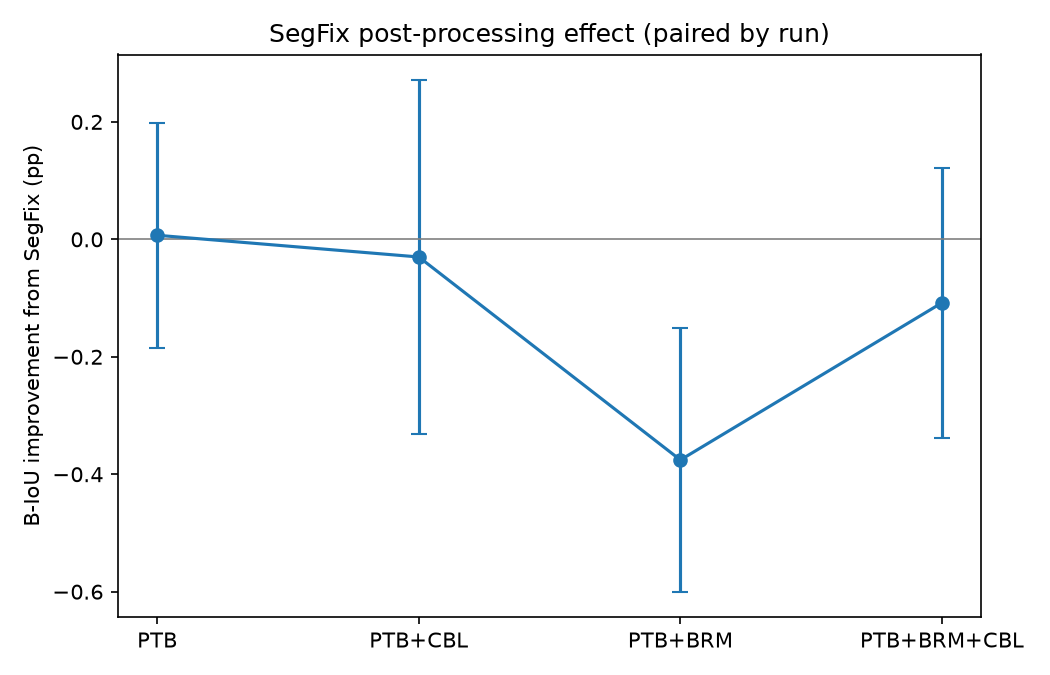
\includegraphics[width=0.7\linewidth]{figures/segfix_delta.png}
\caption{B-IoU improvement from SegFix, paired by run (same checkpoint, with vs.\ without post-processing).}
\end{figure}

\begin{table}[h]
\centering
\resizebox{\textwidth}{!}{\begin{tabular}{lcc}
\toprule
Comparison & B-IoU & mIoU \\
\midrule
PTB + SegFix vs.\ PTB & no detectable effect at $n{=}3$ seeds & no detectable effect at $n{=}3$ seeds \\
PTB+CBL + SegFix vs.\ PTB+CBL & no detectable effect at $n{=}3$ seeds & no detectable effect at $n{=}3$ seeds \\
PTB+BRM + SegFix vs.\ PTB+BRM & no detectable effect at $n{=}3$ seeds & no detectable effect at $n{=}3$ seeds \\
PTB+BRM+CBL + SegFix vs.\ PTB+BRM+CBL & no detectable effect at $n{=}3$ seeds & no detectable effect at $n{=}3$ seeds \\
\bottomrule
\end{tabular}
}
\end{table}

\section{Per-Class Breakdown}

Classes that regress under + PTB + BRM + CBL: Jacket, Hat, Hoodies, Vest, Skirt, TShirt, Hair, Body. Correlation between a class's baseline mean IoU and its baseline seed-to-seed std is -0.67 (lower-IoU classes do show higher seed variance). Classes that regress on B-IoU: Jacket, Hat, Hoodies, Vest, Skirt, TShirt, Hair, Body.

\begin{figure}[h]
\centering
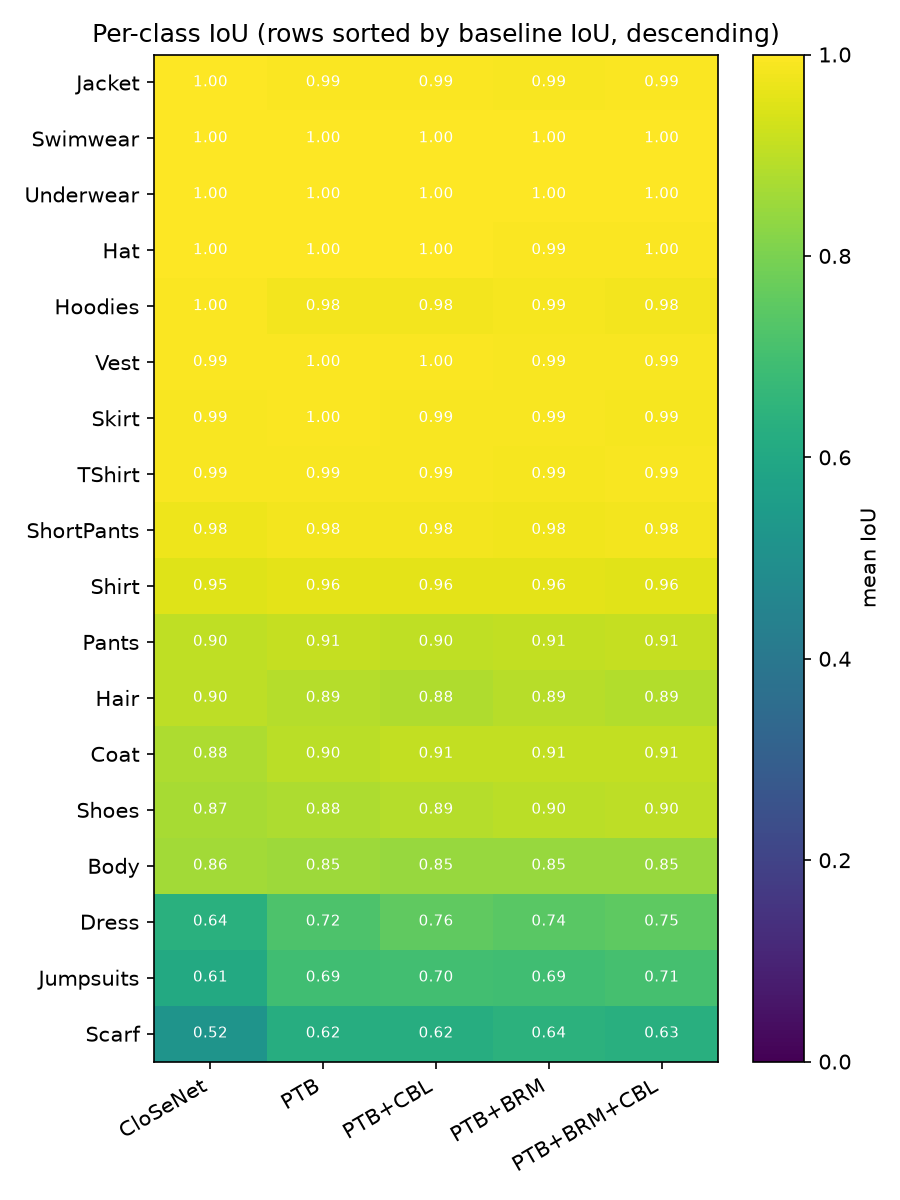
\includegraphics[width=0.65\linewidth]{figures/per_class_heatmap.png}
\caption{Per-class IoU, rows sorted by baseline IoU descending.}
\end{figure}

\begin{figure}[h]
\centering
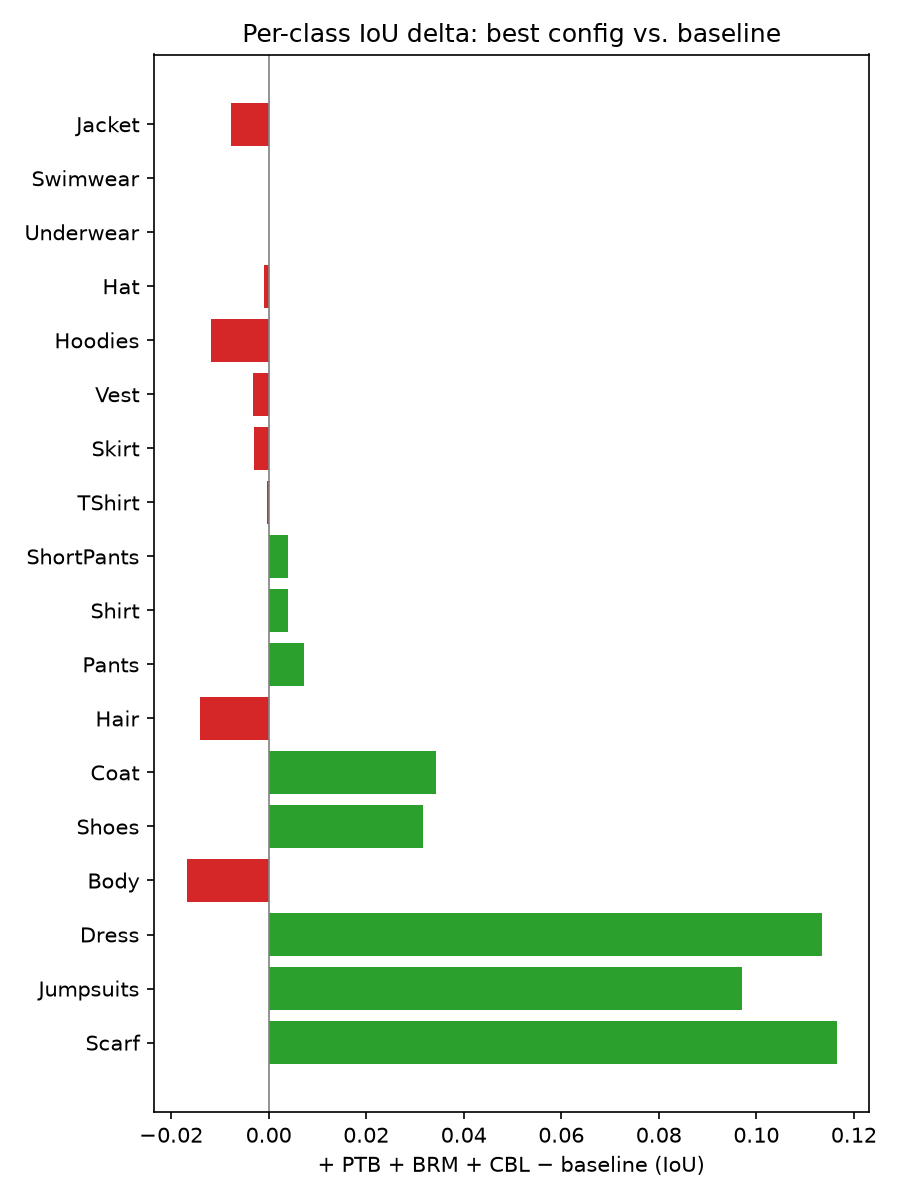
\includegraphics[width=0.65\linewidth]{figures/per_class_delta.png}
\caption{Per-class IoU delta: best config vs.\ baseline.}
\end{figure}

\begin{figure}[h]
\centering
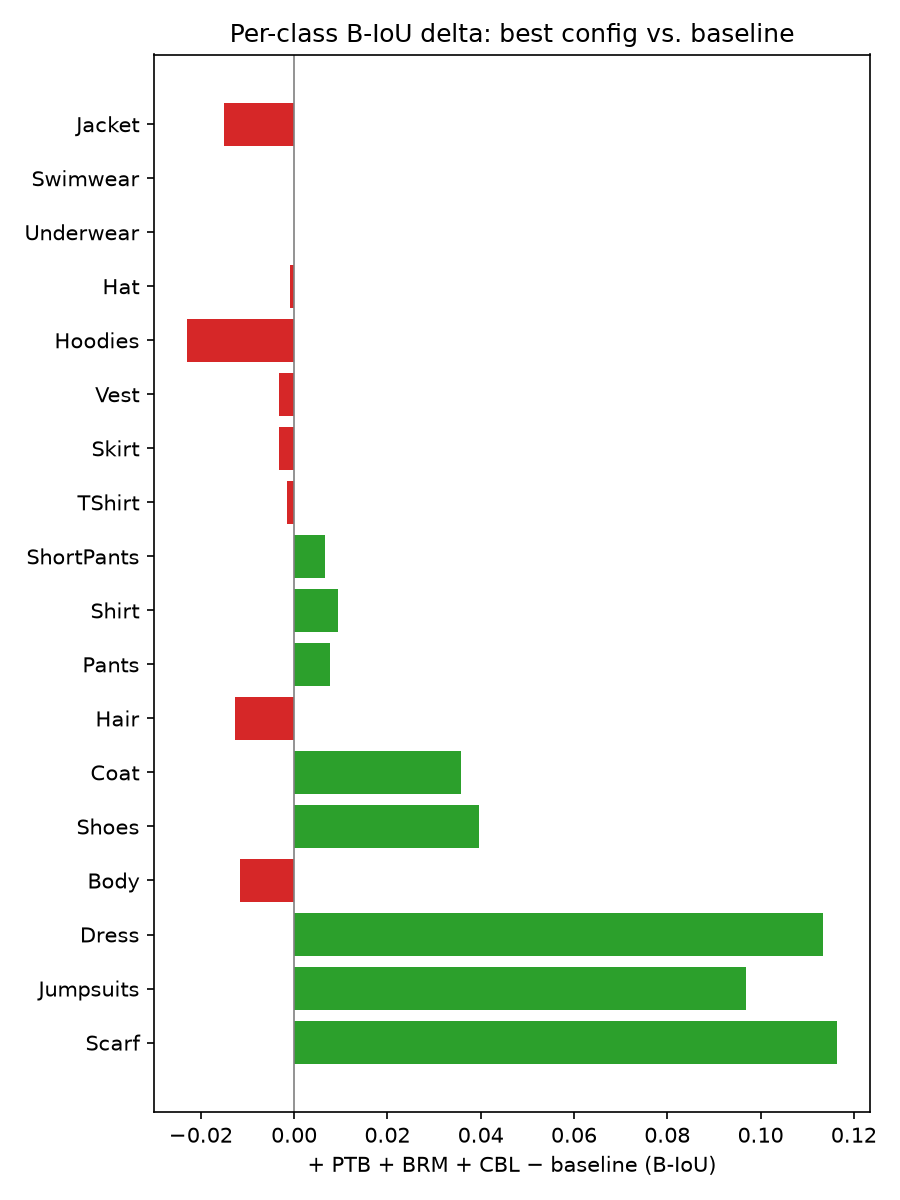
\includegraphics[width=0.65\linewidth]{figures/per_class_delta_biou.png}
\caption{Per-class B-IoU delta: best config vs.\ baseline.}
\end{figure}

\section{Training Dynamics}

Training curves (mean $\pm$ seed std ribbon) for baseline, +CBL, +PTB+CBL, and
+PTB+BRM+CBL. val/cbl\_loss decreases by 0.0695 from start to end of training, evidence CBL is doing something. No config's best checkpoint was selected from a late epoch.

\begin{figure}[h]
\centering
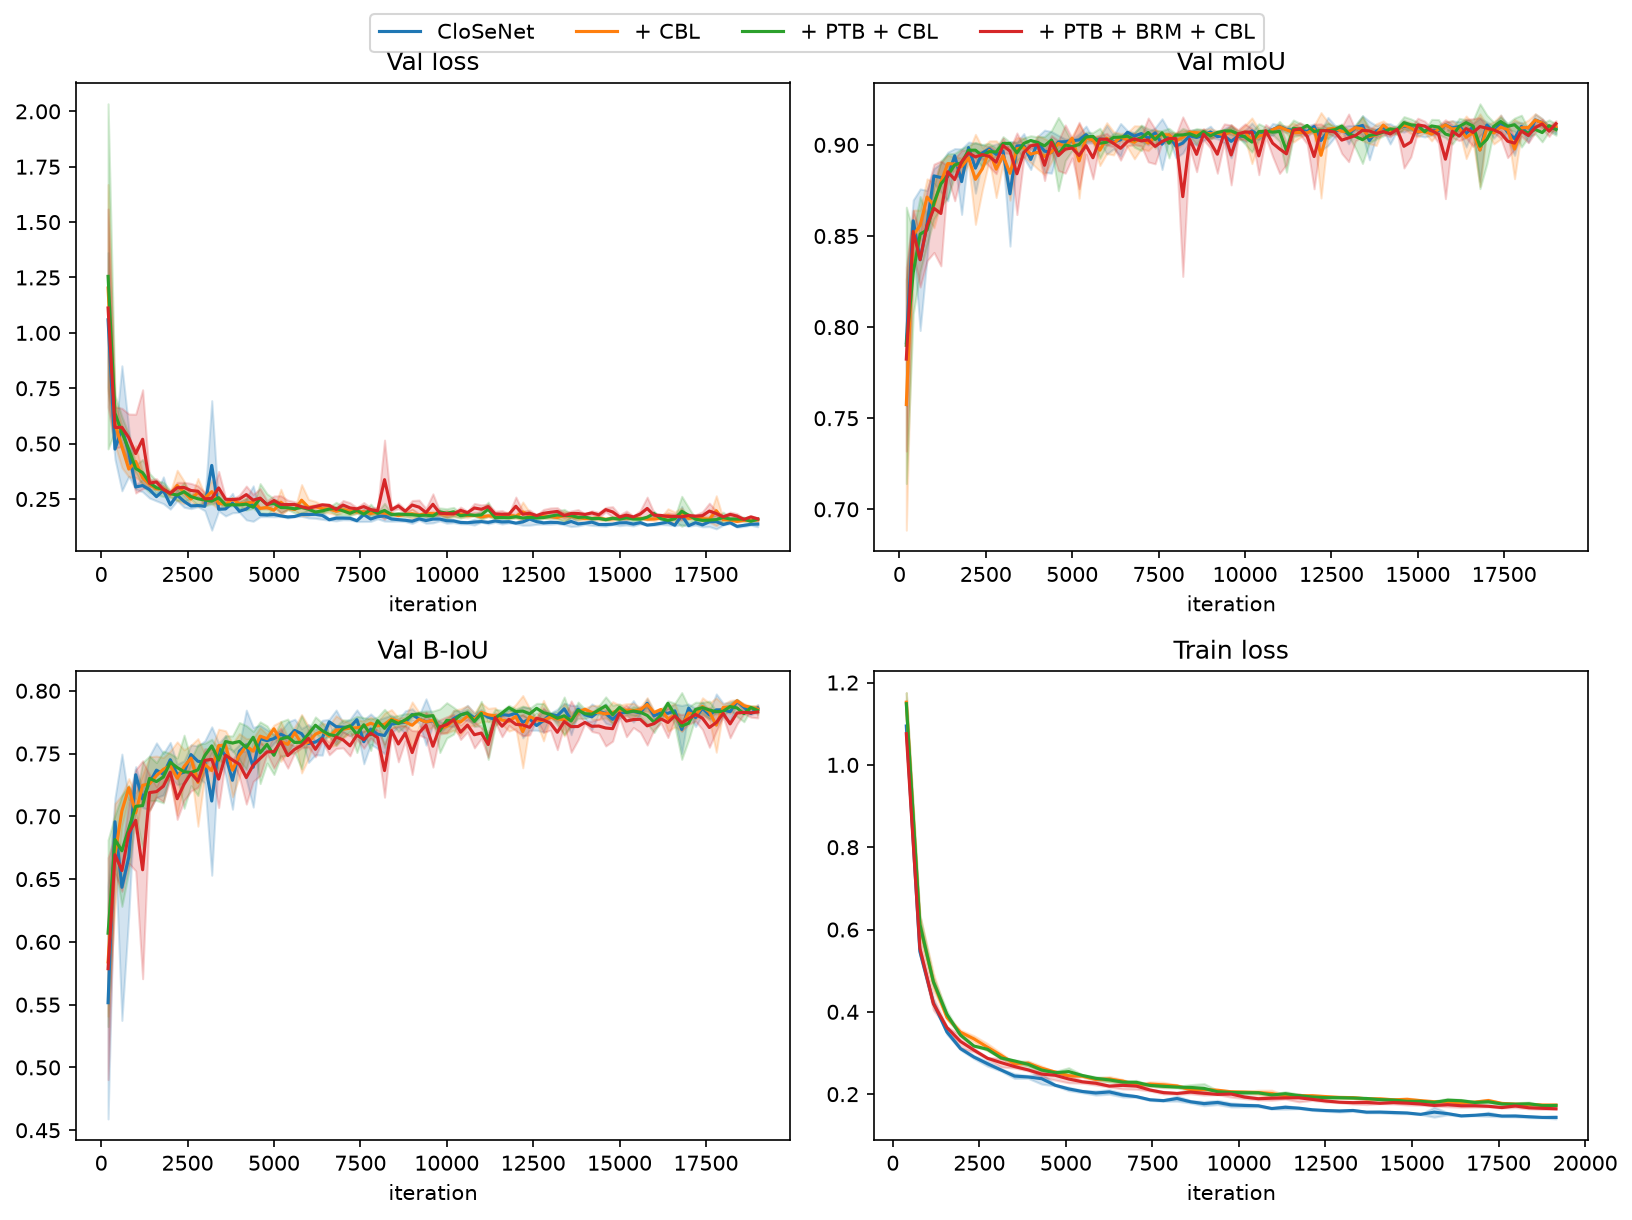
\includegraphics[width=\linewidth]{figures/training_dynamics.png}
\caption{Val loss, val mIoU, val B-IoU, and train loss over training.}
\end{figure}

\begin{table}[h]
\centering
\begin{tabular}{lc}
\toprule
Model & Best-checkpoint epoch \\
\midrule
CloSeNet & 42.7 $\pm$ 6.8 \\
+ CBL & 42.7 $\pm$ 6.8 \\
+ PTB & 42.3 $\pm$ 4.0 \\
+ PTB + SegFix & 42.3 $\pm$ 4.0 \\
+ PTB + CBL & 37.0 $\pm$ 6.6 \\
+ PTB + CBL + SegFix & 37.0 $\pm$ 6.6 \\
+ PTB + BRM & 41.0 $\pm$ 6.2 \\
+ PTB + BRM + SegFix & 41.0 $\pm$ 6.2 \\
+ PTB + BRM + CBL & 38.3 $\pm$ 7.2 \\
+ PTB + BRM + CBL + SegFix & 38.3 $\pm$ 7.2 \\
\bottomrule
\multicolumn{2}{l}{\footnotesize $^\dagger$mean epoch $\geq$ 90\% of max\_epochs (50); may benefit from longer training.} \\
\end{tabular}

\end{table}

\section{Boundary vs.\ Inner Tradeoff}

Do boundary-region improvements come at the cost of inner-region accuracy? Each
point is one (config, seed) run; an ideal method moves points up and to the right
(better at both), while a method trading inner accuracy for boundary accuracy would
move points up and to the left.

\begin{figure}[h]
\centering
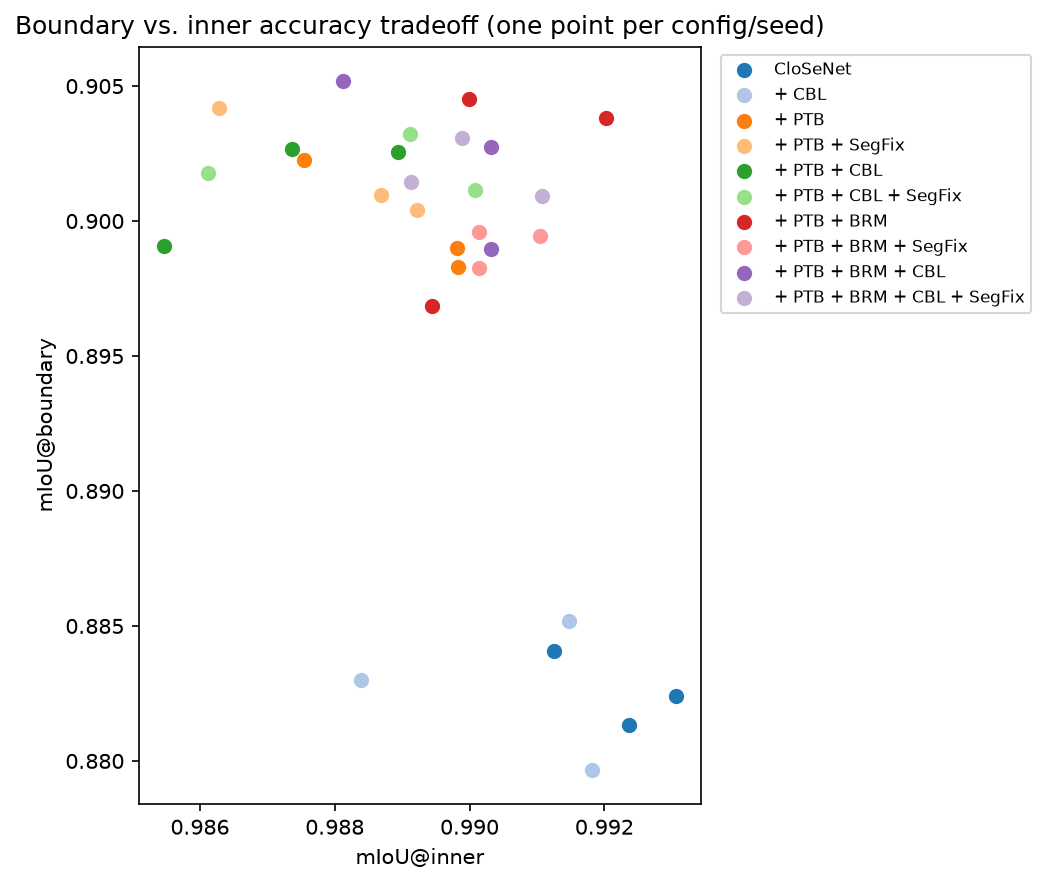
\includegraphics[width=0.75\linewidth]{figures/boundary_inner_scatter.png}
\caption{mIoU@inner vs.\ mIoU@boundary, one point per (config, seed).}
\end{figure}

\end{document}
